\chapter{Annexe}
\label{sec:annexe}
Cette section détaille les résultats présentés à la section \ref{sec:3_jeu_de_donnees_2}.

Les tableaux \ref{tab:2_p}, \ref{tab:2_r} et \ref{tab:2_f} présentent respectivement la précision,
rappel et mesure-F obtenue avec le jeu de données 2 présenté à la section \ref{sec:jeux_de_donnees}.
Les modèles classifient des lectures de $3000$ nucléotides dans $695$ genres. Les meilleurs
résultats de chaque colonne sont marqués en \textbf{gras} et les seconds meilleurs, en

% Tableaux
\begin{table}[hbt!]
\centering
\caption{
    Précision macro pour le jeu de données 2.
}
\begin{tabular}{lccccccc} \hline
       & \multicolumn{7}{c}{Précision macro \%}       \\ \cmidrule(lr){2-8}
Tool             & Domain  & Phylum  & Class   & Order   & Family  & Genus   & Mean \\ \hline
MMSeqs 2         & $98,05$ & $92,62$ & $91,39$ & $83,96$ & $77,91$ & $56,02$ & $83,33$ \\
Kraken 2         & $88,97$ & $71,00$ & $69,91$ & $64,41$ & $60,67$ & $48,49$ & $67,24$ \\
Transformer      & $97,61$ & $81,21$ & $79,54$ & $69,13$ & $63,92$ & $51,55$ & $73,83$\\
Transformer-CNN  & $98,22$ & $88,47$ & $87,63$ & $80,40$ & $75,77$ & $63,77$ & $82,38$ \\
Mamba            & $98,92$ & $93,88$ & $92,67$ & $87,61$ & $83,80$ & $73,28$ & $88,36$ \\
Mamba-Dual       & $99,00$ & $94,67$ & $\mathbf{93,55}$ & $\mathbf{88,97}$ & $84,71$ & $73,36$ & $89,04$ \\
Mamba-CNN        & $\mathit{99,08}$ & $\mathbf{94,87}$ & $\mathit{93,51}$ & $\mathit{88,91}$ & $\mathit{84,76}$ & $\mathit{73,48}$ & $\mathbf{89,10}$ \\
Mamba-Dual-CNN   & $\mathbf{99,20}$ & $\mathit{94,72}$ & $93,34$ & $88,64$ & $\mathbf{84,97}$ & $\mathbf{73,68}$ & $\mathit{89,09}$ \\
\hline
Modèle aléatoire & $50,00$ & $3,85$  & $2,50$  & $0,93$ & $0,46$ & $0,14$  & $9,65$ \\
\hline
\label{tab:2_p}
\end{tabular}
\end{table}

\begin{table}[hbt!]
\centering
\caption{
    Rappel macro pour le jeu de données 2.
}
\begin{tabular}{lccccccc} \hline
       & \multicolumn{7}{c}{Rappel macro \%}       \\ \cmidrule(lr){2-8}
Tool             & Domain  & Phylum  & Class   & Order   & Family  & Genus   & Mean \\ \hline
MMSeqs 2         & $97,95$ & $87,16$ & $86,37$ & $80,35$ & $74,92$ & $55,19$ & $80,32$ \\
Kraken 2         & $89,97$ & $64,76$ & $64,10$ & $59,63$ & $57,65$ & $48,99$ & $64,18$ \\
Transformer      & $95,65$ & $77,85$ & $77,15$ & $67,72$ & $61,58$ & $47,72$ & $71,28$ \\
Transformer-CNN  & $97,51$ & $88,47$ & $87,48$ & $80,63$ & $75,15$ & $62,09$ & $81,89$ \\
Mamba            & $\mathit{98,97}$ & $\mathbf{95,03}$ & $\mathbf{94,05}$ & $\mathit{88,99}$ & $84,56$ & $72,60$ & $\mathit{89,03}$ \\
Mamba-Dual       & $98,86$ & $\mathit{94,98}$ & $93,79$ & $88,65$ & $84,57$ & $\mathit{73,07}$ & $88,99$ \\
Mamba-CNN        & $\mathbf{99,01}$ & $94,81$ & $\mathit{93,94}$ & $88,63$ & $\mathbf{84,65}$ & $73,03$ & $89,01$ \\
Mamba-Dual-CNN   & $98,88$ & $94,82$ & $93,93$ & $\mathbf{89,01}$ & $\mathit{84,61}$ & $\mathbf{73,14}$ & $\mathbf{89,07}$ \\
\hline
Modèle aléatoire & $50,00$ & $3,85$  & $2,50$  & $0,93$ & $0,46$ & $0,14$  & $9,65$ \\
\hline
\label{tab:2_r}
\end{tabular}
\end{table}

\begin{table}[hbt!]
\centering
\caption{
    Mesure-F macro pour le jeu de données 2.
}
\begin{tabular}{lccccccc} \hline
       & \multicolumn{7}{c}{Mesure-F macro \%}       \\ \cmidrule(lr){2-8}
Tool             & Domain  & Phylum  & Class   & Order   & Family  & Genus   & Mean \\ \hline
MMSeqs 2         & $97,99$ & $89,65$ & $88,61$ & $81,92$ & $76,14$ & $55,34$ & $81,61$ \\
Kraken 2         & $89,39$ & $67,00$ & $66,10$ & $61,16$ & $58,41$ & $48,02$ & $65,01$ \\
Transformer      & $96,61$ & $78,70$ & $77,02$ & $66,97$ & $61,20$ & $47,47$ & $71,33$ \\
Transformer-CNN  & $97,86$ & $87,99$ & $87,14$ & $79,95$ & $74,73$ & $61,50$ & $81,53$ \\
Mamba            & $\mathit{98,95}$ & $94,38$ & $93,26$ & $88.11$ & $83.82$ & $72.18$ & $88.45$ \\
Mamba-Dual       & $98,93$ & $\mathit{94,76}$ & $\mathit{93,57}$ & $\mathbf{88,65}$ & $84,39$ & $72,62$ & $88,82$ \\
Mamba-CNN        & $\mathbf{99,04}$ & $\mathbf{94,77}$ & $\mathbf{93,65}$ & $\mathit{88,61}$ & $\mathit{84,43}$ & $\mathit{72,64}$ & $\mathbf{88,86}$ \\
Mamba-Dual-CNN   & $\mathbf{99,04}$ & $94,67$ & $93,49$ & $\mathit{88,61}$ & $\mathbf{84,48}$ & $\mathbf{72,75}$ & $\mathit{88,84}$ \\
\hline
Modèle aléatoire & $50,00$ & $3,85$  & $2,50$  & $0,93$ & $0,46$ & $0,14$  & $9,65$ \\
\hline
\label{tab:2_f}
\end{tabular}
\end{table}

% Niveaux
Les figures \ref{fig:2_n_p}, \ref{fig:2_n_r} et \ref{fig:2_n_f} montrent les performances des
modèles à différents niveaux taxonomiques.

\begin{figure}[hbt!]
  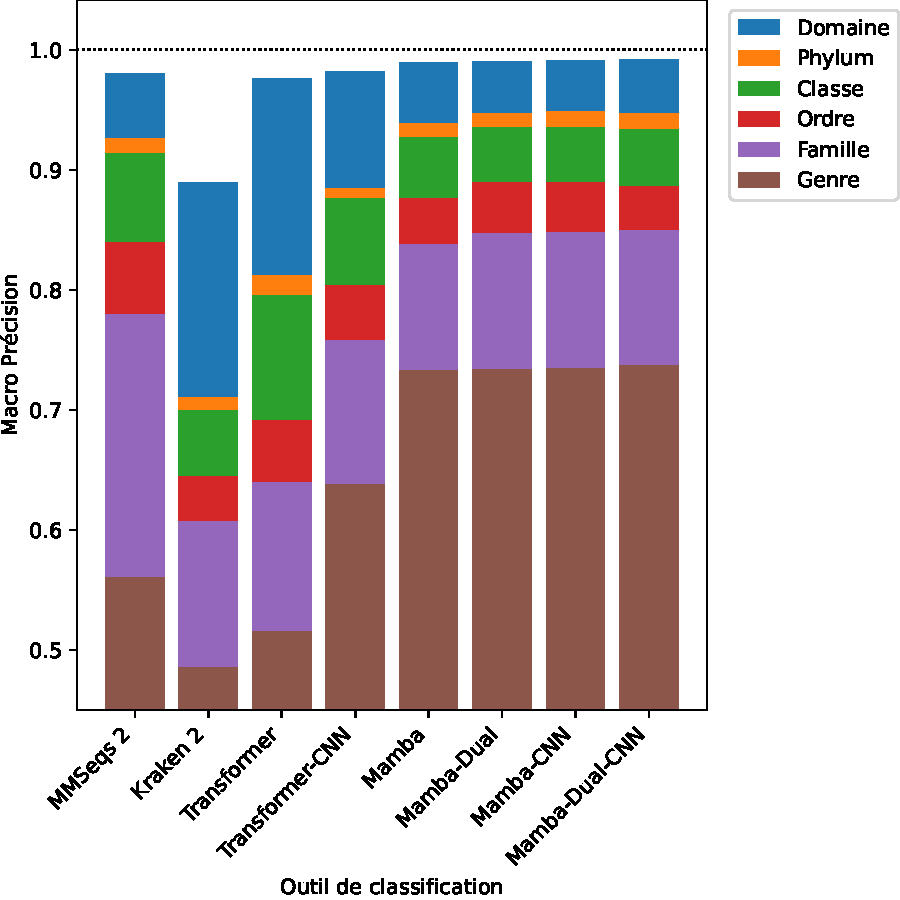
\includegraphics[width=\linewidth]{figures/dataset_2_taxa_Precision.pdf}
  \centering
  \caption{Précision macro à 6 niveaux taxonomiques pour le jeu de données 2}
    \label{fig:2_n_p}
\end{figure}

\begin{figure}[hbt!]
  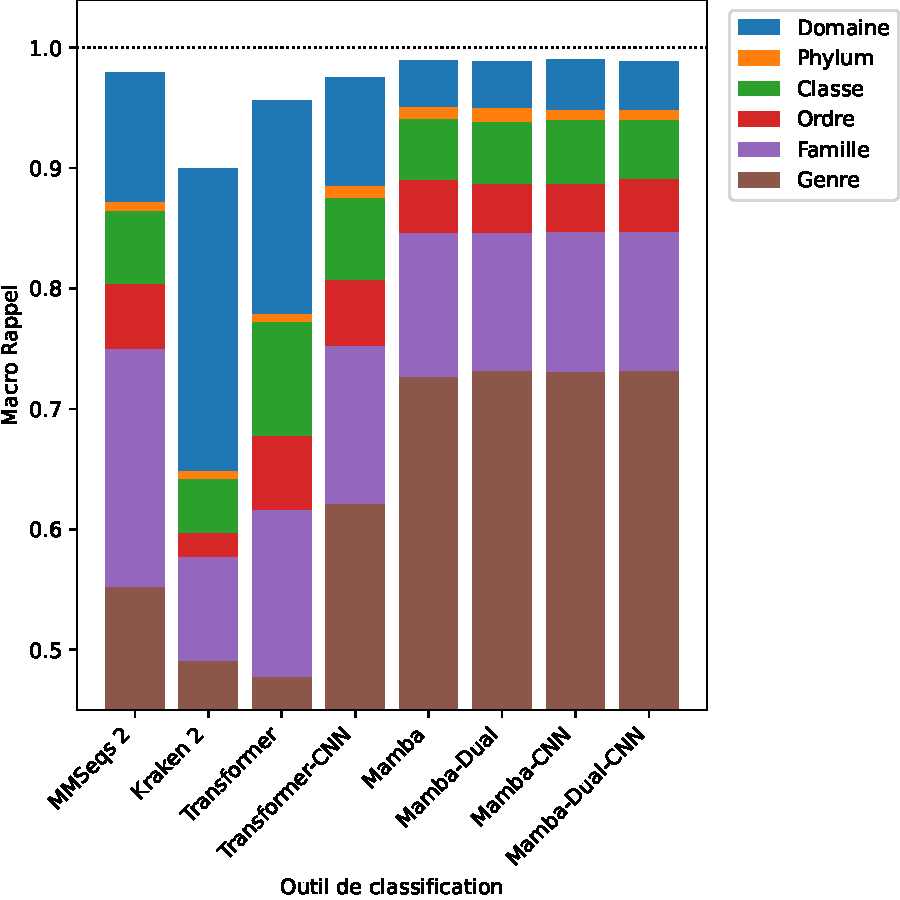
\includegraphics[width=\linewidth]{figures/dataset_2_taxa_Rappel.pdf}
  \centering
  \caption{Rappel macro à 6 niveaux taxonomiques pour le jeu de données 2}
    \label{fig:2_n_r}
\end{figure}

\begin{figure}[hbt!]
  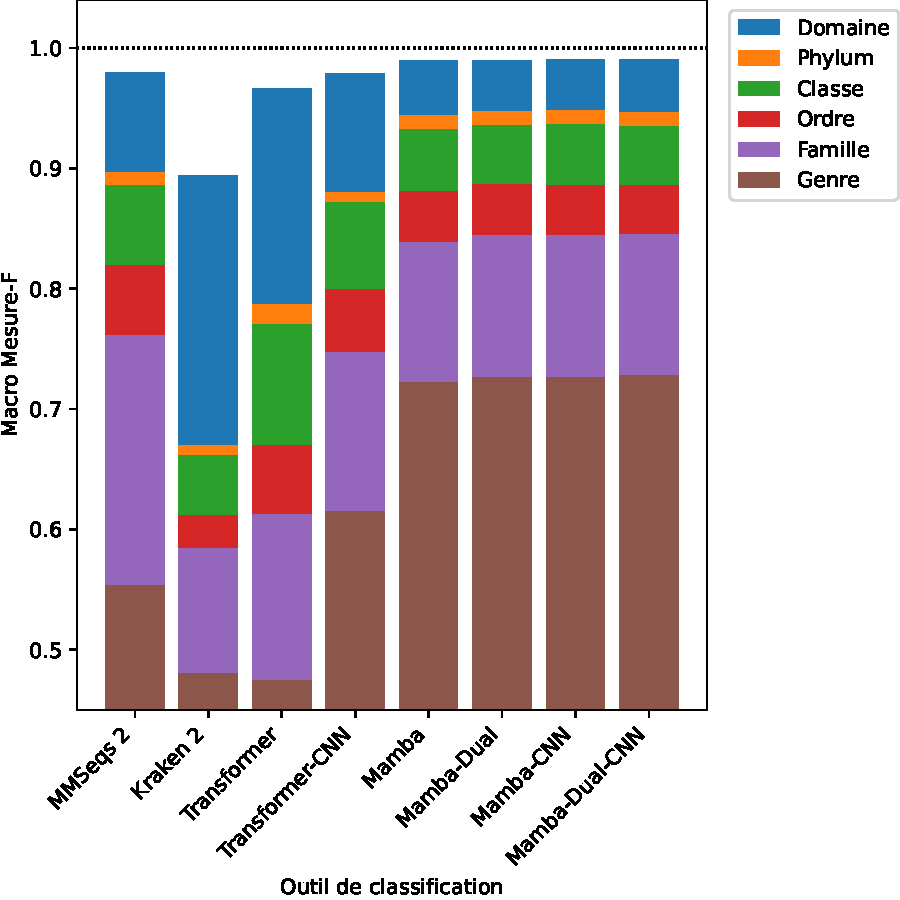
\includegraphics[width=\linewidth]{figures/dataset_2_taxa_Mesure-F.pdf}
  \centering
  \caption{Mesure-F macro à 6 niveaux taxonomiques pour le jeu de données 2}
    \label{fig:2_n_f}
\end{figure}


% Violon
Les figures \ref{fig:2_v_p}, \ref{fig:2_v_r} et \ref{fig:2_v_f} montrent les performances des
modèles à différents niveaux taxonomiques. Les barres horizontales indiquent les médianes.

\begin{figure}[hbt!]
  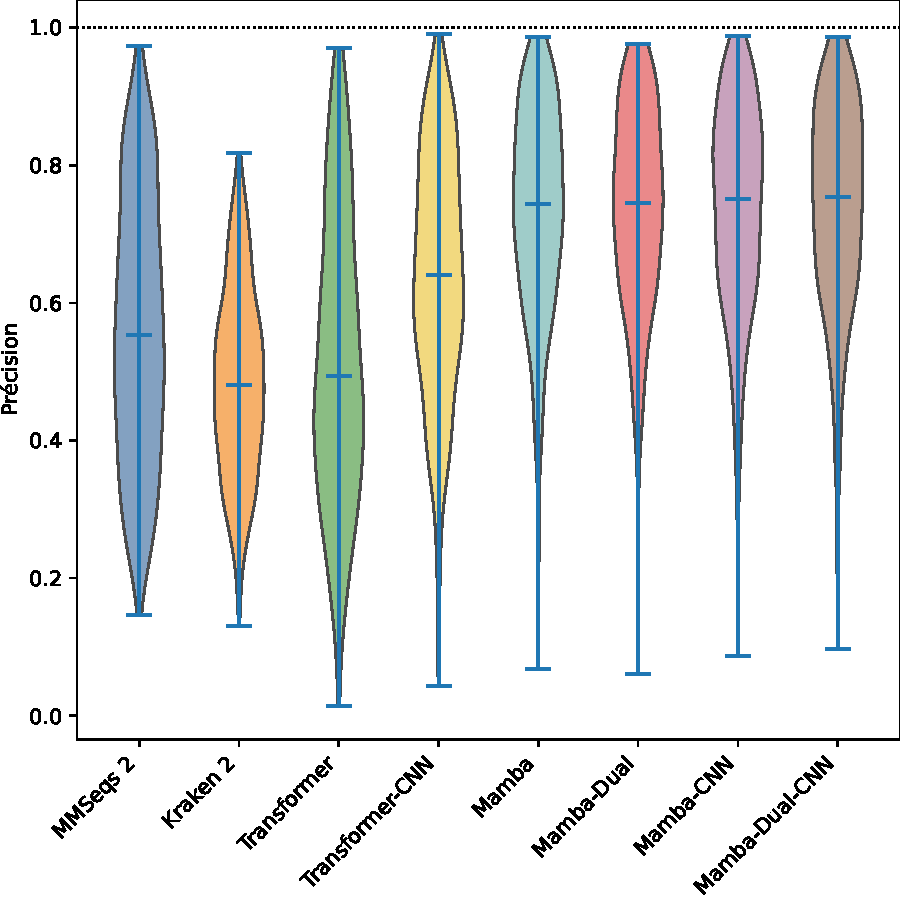
\includegraphics[width=\linewidth]{figures/dataset_2_violinplot_precision.pdf}
  \centering
  \caption{Diagramme violon de la précision macro pour le jeux de données 2}
  \label{fig:2_v_p}
\end{figure}

\begin{figure}[hbt!]
  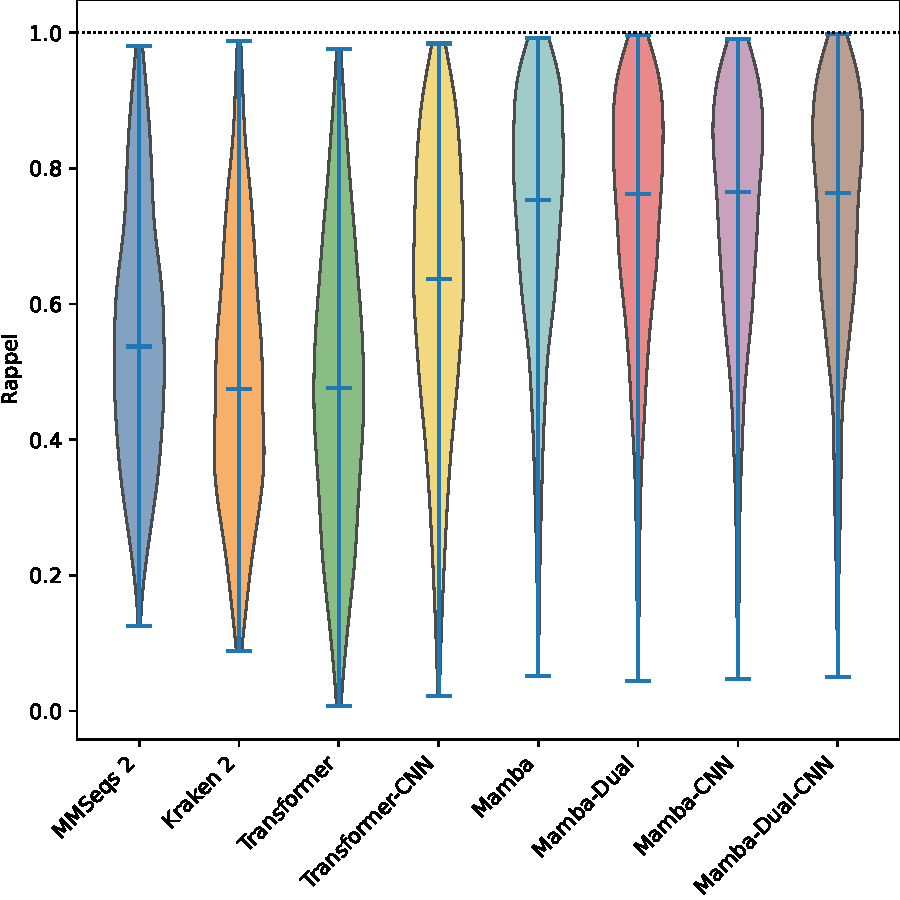
\includegraphics[width=\linewidth]{figures/dataset_2_violinplot_recall.pdf}
  \centering
  \caption{Diagramme violon du rappel macro pour le jeux de données 2}
  \label{fig:2_v_r}
\end{figure}

\begin{figure}[hbt!]
  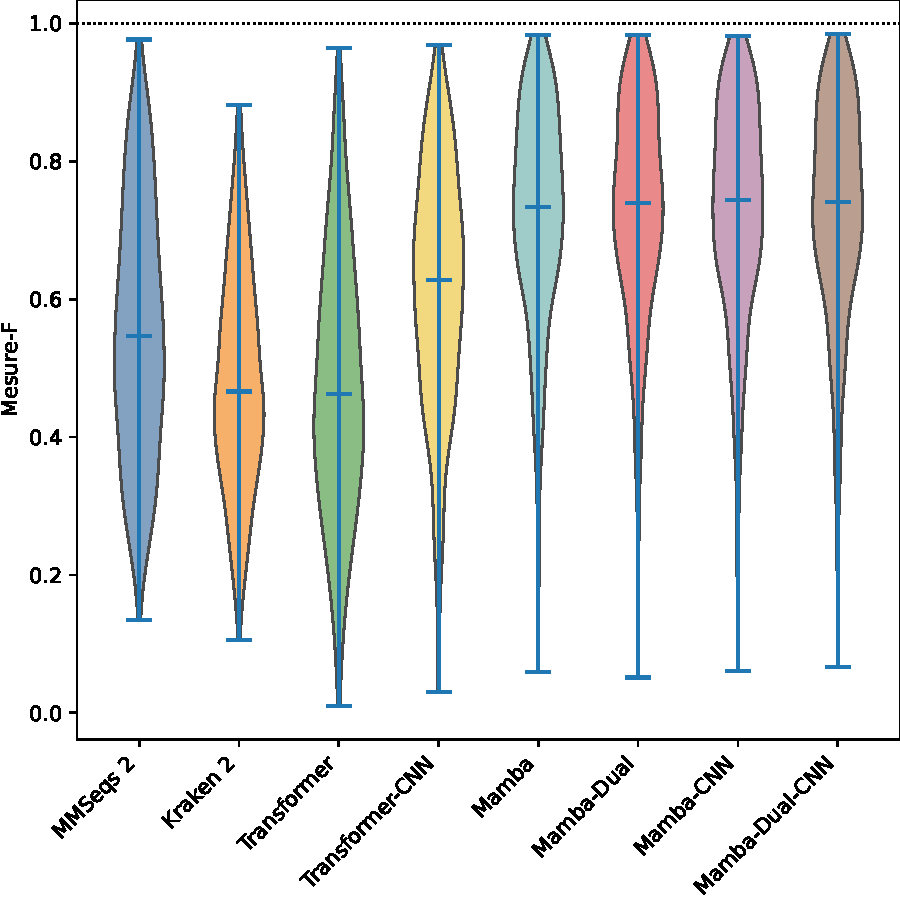
\includegraphics[width=\linewidth]{figures/dataset_2_violinplot_f1.pdf}
  \centering
  \caption{Diagramme violon de la mesure-F macro pour le jeux de données 2}
  \label{fig:2_v_f}
\end{figure}


